\begin{solution}
\begin{enumerate}
\item  We compute
\begin{eqnarray*}
   \norm{f-f_N}^2 &=& \big( f-f_N, f-f_N\big) \\[0.5em]
 &=& \bigg( f - \sum_{n=1}^N c_n \psi_n,
                           f - \sum_{m=1}^N c_m \psi_m\bigg) \\[0.5em]
 &=& \bigg( f - \sum_{n=1}^N c_n \psi_n, f\bigg) 
              - \bigg( f - \sum_{n=1}^N c_n \psi_n,  \sum_{m=1}^N c_m \psi_m\bigg) \\[0.5em]
 &=& (f,f) - \bigg(\sum_{n=1}^N c_n \psi_n, f\bigg) 
              - \bigg( f,  \sum_{m=1}^N c_m \psi_m\bigg) 
              + \bigg(\sum_{n=1}^N c_n \psi_n, \sum_{m=1}^N c_m \psi_m\bigg) \\[0.5em]
 &=& (f,f) - \sum_{n=1}^N c_n (\psi_n, f) 
           - \sum_{m=1}^N c_m (f,\psi_m)
           + \sum_{n=1}^N \sum_{m=1}^N c_n c_m (\psi_n, \psi_m) \\[0.5em]
 &=& (f,f) - \sum_{n=1}^N c_n (\psi_n, f) 
           - \sum_{m=1}^N c_m (f,\psi_m)
           + \sum_{n=1}^N c_n^2  (\psi_n, \psi_n)\\[0.5em]
 &=& (f,f) - \sum_{n=1}^N c_n^2  
           - \sum_{m=1}^N c_m^2 
           + \sum_{n=1}^N c_n^2 \\[0.5em]
 &=& (f,f) - \sum_{n=1}^N c_n^2,
\end{eqnarray*}
where at each equal sign we have use:
(1) the definition of the norm; 
(2) the definition of $f_N$;
(3) linearity of the inner product in the second argument;
(4) linearity of the inner product in the first component;
(5) linear of the inner product;
(6) orthogonality of the eigenfunctions: $(\psi_n,\psi_n) = 0$ if $n\ne m$;
(7) $(f,\psi_n) = (\psi_n,f) = c_n$ and $(\psi_n,\psi_n) = 1$;
(8) simple algebra.
\item Code and the plot follow at the end of the problem.

\item You can work out this equality for the specific case of
$u(x) = x(1-x)/2$.  One computes (e.g., in Mathematica) that
\[ (u, \psi_n) = (x(1-x)/2,\psi_n) = \left\{
    \begin{array}{ll}
       {\displaystyle{2 \sqrt{2} \over n^3 \pi^3},}& \mbox{$n$ odd;}\\[.75em]
       0, & \mbox{$n$ even}. 
    \end{array}\right. \]
This formula for $(u,\psi_n) = (u,\psi_n)/(\psi_n,\psi_n)$ 
exactly matches $c_n/\lambda_n$.   This calculation is all that
is needed for full credit.

Alternatively, one can show that this result holds \emph{in general}.
Notice that since $Lu = f$ and $L$ is symmetric, we have
\[ c_n = {(f,\psi_n)\over (\psi_n,\psi_n)} 
       = {(Lu,\psi_n)\over (\psi_n,\psi_n)}
       = {(u,L\psi_n)\over (\psi_n,\psi_n)}
       = {(u,\lambda_n \psi_n)\over (\psi_n,\psi_n)}
       = \lambda_n {(u,\psi_n)\over (\psi_n,\psi_n)},\]
which is equivalent to the given statement.
       


\item The requested plot for (b) and (d) is shown below. 

\begin{center}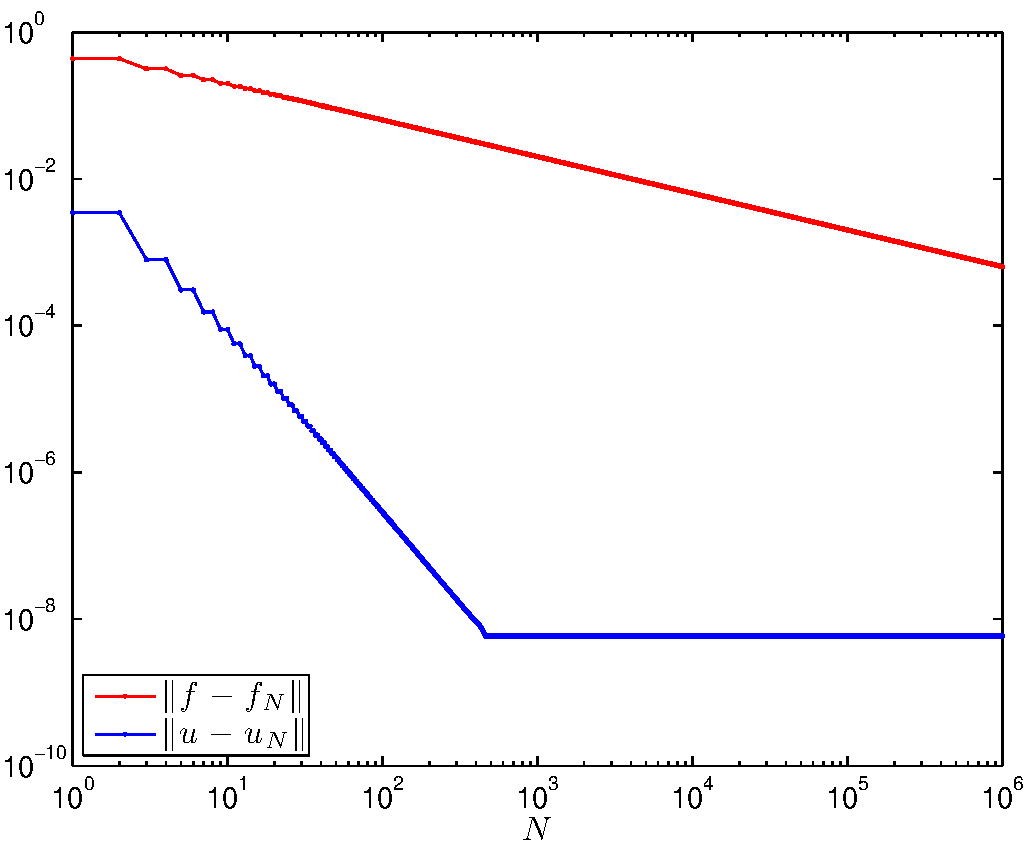
\includegraphics[scale=0.7]{fourerr}\end{center}
\end{enumerate}

The code that produced the plot above for (b) and (c) is shown below.

{\small \begin{verbatim}
 n = [1:1e6]';
 cn = (sqrt(2)/pi)*(1+(-1).^(n+1))./(n);
 lamn = pi^2*n.^2;
 normf2 = 1;
 normu2 = 1/120;
 figure(1), clf
 loglog([1:length(cn)], sqrt(normf2-cumsum(cn.^2)),'r.-')
 hold on
 loglog(n, sqrt(normu2-cumsum((cn./lamn).^2)),'b.-')

 set(gca,'fontsize',14)
 xlabel('$N$','fontsize',16,'interpreter','latex')
 legend('$\|f-f_N\|$','$\|u-u_N\|$',3)
 set(legend,'interpreter','latex','fontsize',16)
 print -depsc2 fourerr
\end{verbatim}}

\end{solution}
